\documentclass{ctexart}
\usepackage{geometry}
\usepackage{array}
\usepackage{makecell}
\usepackage{enumitem}
\usepackage{booktabs}
\usepackage{ragged2e}
\usepackage{tabularx}
\usepackage{fancyhdr} % 用于自定义页眉页脚
\usepackage{graphicx} % 应该已存在 (如果之前添加过)
\usepackage[HTML]{xcolor} % 新增：用于颜色定义和 colorbox
\usepackage{emptypage} % 如果之前添加了用于移除末尾空白页，请保留

% 页面边距设置
\geometry{a4paper, margin=1in}

% 自定义表格列类型
\newcolumntype{L}[1]{>{\RaggedRight\arraybackslash}p{#1}} % 左对齐，自动换行
\newcolumntype{M}[1]{>{\centering\arraybackslash}m{#1}}  % 水平居中，垂直居中，自动换行 (用户定义)

% fancyhdr 设置
\pagestyle{fancy} % 应用 fancy 页面样式
\fancyhf{} % 清空所有页眉页脚设置
\fancyhead[L]{\nouppercase{\leftmark}} % 页眉左侧显示当前节标题
\fancyfoot[C]{\thepage} % 页脚中间显示页码
\renewcommand{\headrulewidth}{0.4pt} % 页眉下方加一条线
\renewcommand{\footrulewidth}{0pt}  % 页脚上方不加线

% 为朴素页面样式（如目录页）重新定义
\fancypagestyle{plain}{%
  \fancyhf{}%
  \fancyfoot[C]{\thepage}%
  \renewcommand{\headrulewidth}{0pt}%
  \renewcommand{\footrulewidth}{0pt}%
}

% 定义横幅颜色
\definecolor{MyBannerColor}{HTML}{0078D7} % 修改为蓝色

\begin{document}

\begin{titlepage}
    \thispagestyle{empty} % 标题页不显示页眉页脚
    \vspace*{-1.15in} % 新增：向上移动1英寸以抵消顶部边距
    % 顶部图片: 设置为铺满整个纸张宽度
    \noindent\hspace*{-1in}%
    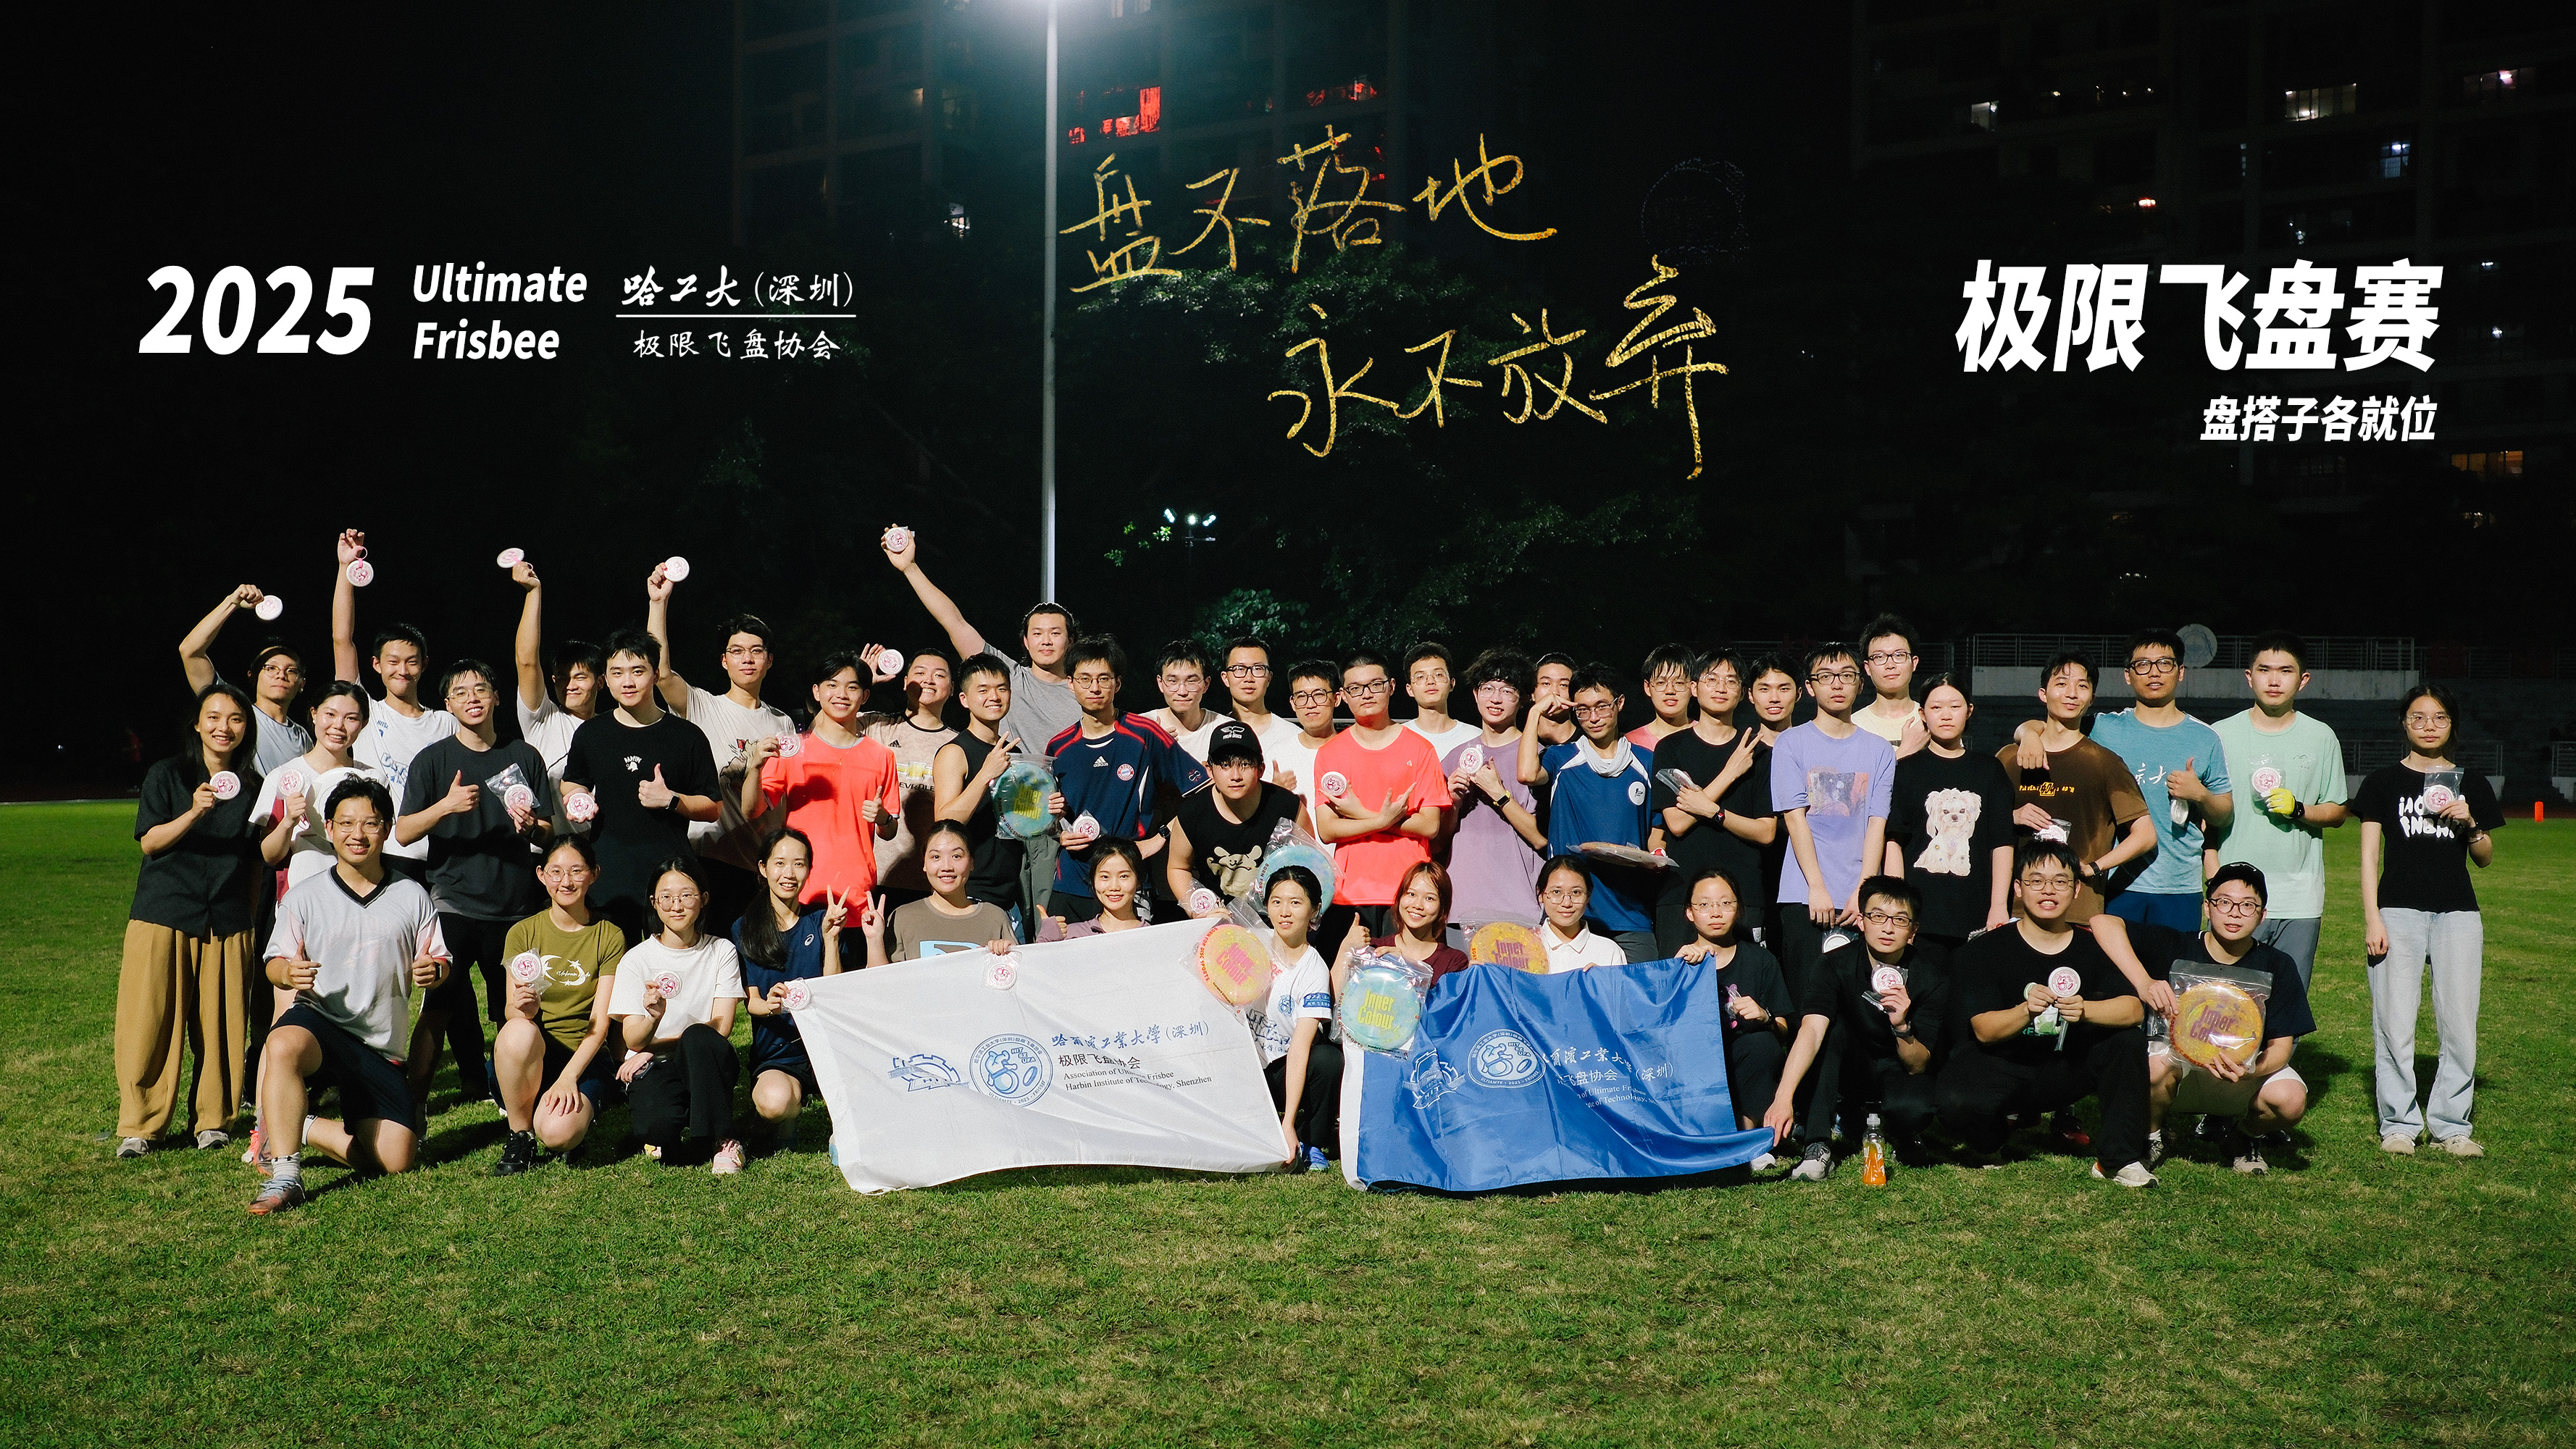
\includegraphics[width=\paperwidth, height=0.4\paperheight, keepaspectratio]{大合照.jpg}%

    % 彩色条带 (无文字，宽度为 paperwidth)
    \vspace{-1pt} % 此行用于消除图片和彩带间的微小间距，应保留
    \noindent\hspace*{-1in}%
    \colorbox{MyBannerColor}{% % 使用您最终确定的颜色名称
        \begin{minipage}[c][2em][c]{\dimexpr\paperwidth-2\fboxsep\relax} % 彩色条带高度，例如3em，宽度为paperwidth
            \hspace{0pt} % 确保minipage有内容以正确计算高度
        \end{minipage}%
    }

    % 彩色条带下方的文本信息
    \begin{center}
        \vspace{4em} % 彩色条带与主标题之间的间距
        {\LARGE 哈尔滨工业大学（深圳）2026体育文化节极限飞盘赛\par} % 主标题移到此处
        
        \vspace{1.5em} % 主标题与副标题之间的间距
        {\Large 赛程安排与注意事项 (5月23日, 5月30日)} \\[2em] % 副标题
        
        {哈尔滨工业大学（深圳）极限飞盘协会} \\[1em]
        {2026年5月8日}\par

        \vspace{12em} % 在日期和旗帜之间添加一些垂直间距
        % 插入修剪后的协会旗帜 PDF
        
\includegraphics[width=0.65\paperwidth, trim=50bp 6.4cm 50bp 6.3cm, clip]{协会旗帜.pdf}
    \end{center}

    \vfill
\end{titlepage}

\clearpage
\pagenumbering{roman}
\pagestyle{plain}
% \tableofcontents
\clearpage
\pagenumbering{arabic}
\pagestyle{fancy}

\section{赛事简介、赛制与场地说明}
本次极限飞盘比赛采用4队积分赛加决赛轮的赛制，旨在为同学们提供充分的交流和竞技机会。
\begin{itemize}
    \item \textbf{参赛队伍：} A队, B队, C队, D队。
    \item \textbf{赛事日程：} 分为2个活动日（5月23日、5月30日15:30-18:30）进行。
    \item \textbf{积分赛与决赛：} 所有队伍两两之间进行一场比赛，共6场积分赛；积分赛后根据积分排名进行三四名及冠亚军决赛。
    \item \textbf{比赛用时与规则：}5人制，上场比例2男3女或3男2女，采取ABBAA规则；每场比赛时长50分钟，抢11分。
    \item \textbf{排位规则：} 积分赛结束后，根据各队积分进行排名。胜一场积2分，平一场积1分，负一场积0分。若积分相同，则依次比较：1) 相互间胜负关系（仅同分队伍间适用）；2) 总净胜分；3) 总得分数。
    \item \textbf{队伍颜色：} 为确保比赛中队伍区分清晰，每场比赛将为对阵双方指定深/浅色队服。请所有参赛队员务必\textbf{准备好深色（建议为黑色或深蓝色）和浅色（建议为白色）运动上衣各一件}。
    \item \textbf{比赛地点与场地安排：}
    \begin{itemize}
        \item \textbf{比赛地点：} 哈工大操场。
        \item \textbf{场地设置：} 使用操场上的两个场地同时进行比赛。
        \begin{itemize}
            \item \textbf{场地1：} 位于靠近维也纳酒店一侧。
            \item \textbf{场地2：} 位于远离维也纳酒店一侧。
        \end{itemize}
    \end{itemize}
\end{itemize}

\newpage

\section{第一活动日：2026年5月23日 - 积分赛 (第1-4场)}

\subsection*{赛程安排 (5月23日)}
\renewcommand{\arraystretch}{1.8}
\begin{tabularx}{\textwidth}{@{} L{2.2cm} L{1.5cm} X L{3.2cm} @{}}
    \toprule
    \textbf{时间段} & \textbf{场地} & \textbf{对阵双方 (左队深色, 右队浅色)} & \textbf{阶段 / 备注} \\
    \midrule
    \multicolumn{4}{l}{\textit{15:30 - 16:00 签到、到场、热身准备}} \\
    \addlinespace
    \multicolumn{4}{c}{\textbf{第一轮积分赛}} \\
    16:00 - 16:50 & 场地1 & A队 (深) vs B队 (浅) & 积分赛第1场 (50分钟) \\
    16:00 - 16:50 & 场地2 & C队 (深) vs D队 (浅) & 积分赛第2场 (50分钟) \\
    \addlinespace
    \multicolumn{4}{l}{\textit{16:50 - 17:10 场间休息、更换衣服 (20分钟)}} \\
    \addlinespace
    \multicolumn{4}{c}{\textbf{第二轮积分赛}} \\
    17:10 - 18:00 & 场地1 & A队 (深) vs D队 (浅) & 积分赛第3场 (50分钟) \\
    17:10 - 18:00 & 场地2 & C队 (深) vs B队 (浅) & 积分赛第4场 (50分钟) \\
    \addlinespace
    \multicolumn{4}{l}{\textit{18:00 - 18:30 Circle交流、队伍总结与自由拉盘}} \\
    \addlinespace
    \bottomrule
\end{tabularx}
\renewcommand{\arraystretch}{1.0}

\subsection*{当日重要提醒 (5月23日)}
\begin{itemize}
    \item 请所有队伍于 15:30 前到达场地签到、热身。到场先签风险告知书,每队一份。
    \item \textbf{重要服装提示：} 本日比赛颜色分配请严格参照上表，左队深色，右队浅色。
\end{itemize}

\newpage

\section{第二活动日：2026年5月30日 - 积分赛(第5-6场) 与 决赛轮}

\subsection*{赛程安排 (5月30日)}
\renewcommand{\arraystretch}{1.8}
\begin{tabularx}{\textwidth}{@{} L{2.2cm} L{1.5cm} X L{3.2cm} @{}}
    \toprule
    \textbf{时间段} & \textbf{场地} & \textbf{对阵双方 (左队深色, 右队浅色)} & \textbf{阶段 / 备注} \\
    \midrule
    \multicolumn{4}{l}{\textit{15:30 - 16:00 签到、到场、热身准备}} \\
    \addlinespace
    \multicolumn{4}{c}{\textbf{第三轮积分赛}} \\
    16:00 - 16:50 & 场地1 & A队 (深) vs C队 (浅) & 积分赛第5场 (50分钟) \\
    16:00 - 16:50 & 场地2 & B队 (深) vs D队 (浅) & 积分赛第6场 (50分钟) \\
    \addlinespace
    \multicolumn{4}{l}{\textit{16:50 - 17:10 场间休息、比分统计、公布决赛排位、更换衣服 (20分钟)}} \\
    \addlinespace
    \multicolumn{4}{c}{\textbf{决赛轮}} \\
    17:10 - 18:00 & 场地1 & 积分排位第3名 vs 第4名 & \textbf{三四名决赛} (50分钟) \\
    17:10 - 18:00 & 场地2 & 积分排位第1名 vs 第2名 & \textbf{冠军决赛} (50分钟) \\
    \addlinespace
    \multicolumn{4}{l}{\textit{18:00 - 18:30 Circle交流、颁奖仪式、合影留念}} \\
    \addlinespace
    \bottomrule
\end{tabularx}
\renewcommand{\arraystretch}{1.0}

\subsection*{当日重要提醒 (5月30日)}
\begin{itemize}
    \item 请所有队伍于 15:30 前到达场地签到、热身。
    \item 决赛轮将决定最终的冠、亚、季、殿军。
    \item 比赛全部结束后请大家不要离开，我们将举办颁奖仪式并拍摄全体大合影！
\end{itemize}

\newpage

\section{赛事总体注意事项}
\begin{enumerate}[label=\arabic*., itemsep=0.5em]
    \item \textbf{参赛服装：} 请所有参赛队员务必\textbf{准备深色和浅色运动上衣各一件}。每场比赛的具体颜色分配请严格参照赛程表。
    \item \textbf{饮水：} 场地不提供一次性水杯，请各位选手\textbf{务必自带水壶及充足饮用水}。
    \item \textbf{安全第一：} 请大家在比赛中务必注意自身和他人的安全，热身充分，量力而行，避免受伤。
    \item \textbf{保险：} 请所有运动员务必提前购买运动保险。
    \item \textbf{准时与场地：} 请各队严格遵守比赛时间，提前到场准备。
    \item \textbf{体育精神：} 秉持"Spirit Of The Game (SOTG)"飞盘精神，尊重比赛，尊重对手，尊重队友，公平竞争。
    \item \textbf{场地保持：} 请爱护场地设施，比赛结束后自觉清理垃圾，保持场地整洁。
\end{enumerate}

\vspace{1.5em}
\begin{center}
期待各位的积极参与，预祝比赛顺利，大家玩得开心！
\end{center}

\noindent\rule{\linewidth}{0.4pt}
\vspace{1em}

\begin{flushleft}
\textbf{主办单位：} \\
哈尔滨工业大学（深圳）团委 \\[1em]

\textbf{承办单位：} \\
哈尔滨工业大学（深圳）极限飞盘协会
\end{flushleft}

\newpage

\appendix
\section{参赛人员名单}

\subsection*{A队}
\renewcommand{\arraystretch}{1.2}
\begin{tabularx}{\textwidth}{@{} L{4.5cm} M{1.4cm} L{3cm} X @{}}
    \toprule
    \textbf{姓名} & \textbf{性别} & \textbf{学号} & \textbf{盘龄} \\
    \midrule
    吴承沣 & 男 & - & 2年以上 \\
    康钊源 & 男 & 2024311150 & 1-2年 \\
    黄家骏 & 男 & 2024311040 & 1-2年 \\
    寇家辉 & 男 & 2024311312 & 6月-1年 \\
    王俊杰 & 男 & 2024312042 & 6月以内 \\
    吴智杰 & 男 & 2510082093 & 6月以内 \\
    罗梦恬 & 女 & 2023311801 & 2年以上 \\
    潘秀丽 & 女 & 2024312180 & 6月以内 \\
    樊黎硕 & 女 & 25S153056 & 6月以内 \\
    肖叶萱 & 女 & 2023215045 & 6月以内 \\
    \bottomrule
\end{tabularx}

\subsection*{B队}
\renewcommand{\arraystretch}{1.2}
\begin{tabularx}{\textwidth}{@{} L{4.5cm} M{1.4cm} L{3cm} X @{}}
    \toprule
    \textbf{姓名} & \textbf{性别} & \textbf{学号} & \textbf{盘龄} \\
    \midrule
    刘慕实 & 男 & 25S151141 & 2年以上 \\
    张骋旭 & 男 & - & 2年以上 \\
    赵浩帆 & 男 & 25B965005 & 6月-1年 \\
    梁柱政 & 男 & 25S154067 & 6月-1年 \\
    杨鸿鑫 & 男 & 2024312706 & 6月以内 \\
    金圣博 & 男 & 210810404 & 6月以内 \\
    Ocean & 女 & 2025213750 & 1-2年 \\
    陈子瑶 & 女 & 2025310432 & 6月以内 \\
    杨千凝 & 女 & 25S164067 & 6月以内 \\
    傅春颖 & 女 & - & - \\
    \bottomrule
\end{tabularx}

\subsection*{C队}
\renewcommand{\arraystretch}{1.2}
\begin{tabularx}{\textwidth}{@{} L{4.5cm} M{1.4cm} L{3cm} X @{}}
    \toprule
    \textbf{姓名} & \textbf{性别} & \textbf{学号} & \textbf{盘龄} \\
    \midrule
    黄家乐 & 男 & - & 2年以上 \\
    马荣 & 男 & 2025330524 & 6月-1年 \\
    金珉宇 & 男 & 2024311060 & 6月以内 \\
    典珅司 & 男 & 2024311045 & 6月以内 \\
    Abdul Quader & 男 & - & 6月以内 \\
    张豫艳 & 女 & - & 2年以上 \\
    EL MOUDDEN ZAYNAB & 女 & 2025330187 & 6月以内 \\
    李焱 & 女 & 25s155079 & 6月以内 \\
    小午 & 女 & 2410012101 & 6月以内 \\
    \bottomrule
\end{tabularx}

\subsection*{D队}
\renewcommand{\arraystretch}{1.2}
\begin{tabularx}{\textwidth}{@{} L{4.5cm} M{1.4cm} L{3cm} X @{}}
    \toprule
    \textbf{姓名} & \textbf{性别} & \textbf{学号} & \textbf{盘龄} \\
    \midrule
    王硕 & 男 & - & 2年以上 \\
    耿增越 & 男 & 2023311226 & 1-2年 \\
    温岩 & 男 & 2024312297 & 6月以内 \\
    万一鸣 & 男 & 2025310507 & 6月以内 \\
    张梦辉 & 男 & 2025312884 & 6月以内 \\
    孟欣 & 女 & 24B926002 & 6月-1年 \\
    段绚涵 & 女 & 2025310723 & 6月以内 \\
    summer & 女 & 2410053014 & 6月以内 \\
    \bottomrule
\end{tabularx}

\end{document}
